\chapter{エネルギーとハミルトニアン}

\lectureoverview{まず能動的対称性の意味を明確にし、並進と回転がどのように運動量と角運動量を生み出すかを復習する。欠けている保存則はエネルギーである。その対称性は時間並進であり、保存量はハミルトニアン\(H=\sum_i p_i\dot q_i-L\)である。この導出はまた、陽な時間依存性がどのようにして選ばれた部分系とその環境の間でエネルギーを移動させるかを正確に示す。}

\section{形式的議論の前の質問}

これから続く主題に必要な古典力学の最低限に近づいているが、なお学ぶ価値のある力学はまだ多く残っている。主要な議論が始まる前に二つの質問が出た。

\begin{classroomqa}
  \audiencequestion{この入門コースの後にはどの本が役に立ちますか。
  \lecturetimestamp{00:00:36--00:02:13}}
  \lecturerresponse{定評のある上級向け参考書はハーバート・ゴールドスタインの\emph{古典力学}である。コーネリアス・ランチョシュの力学の変分原理に関する本もまた関連する資料である。一人の講師があらゆる利用可能な教科書を概観できると装うよりも、授業の読書リストの方が役に立つ。}
\end{classroomqa}

二番目の質問は、未解決の測定の歴史におけるある時点を記録している。2011年にOPERA実験は、CERNからグラン・サッソへ送られたニュートリノが明らかに早く到着したと報告していた。報告されたずれはニュートリノを生成するために用いた陽子パルスより短かったので、時間解析は、放出時に一つのニュートリノに印を付け検出時に同じ粒子を認識するのではなく、パルス波形を比較することに依存していた。

\begin{classroomqa}
  \audiencequestion{見かけ上の超光速ニュートリノの結果は解決されていたのですか。
  \lecturetimestamp{00:02:30--00:09:03}}
  \lecturerresponse{そのときには結論を正当化できなかった。ビームパルスの形状、標的の加熱、同期のすべてが技術的な精査を必要とした。一つの推測的な提案はGPS衛星の運動を考慮した。衛星の座標系では、タイミング信号が伝わる間に線源と検出器が動き、数十ナノ秒程度の補正が生じる。その見積もりは桁の練習として興味深かったが、実験の信頼できる診断として提示されたものではなかった。関連する速度での通常のローレンツ収縮は、報告された効果を与えるには小さすぎた。適切な対応は実験解析を待つことであった。}
\end{classroomqa}

\begin{figure}[htbp]
  \centering
  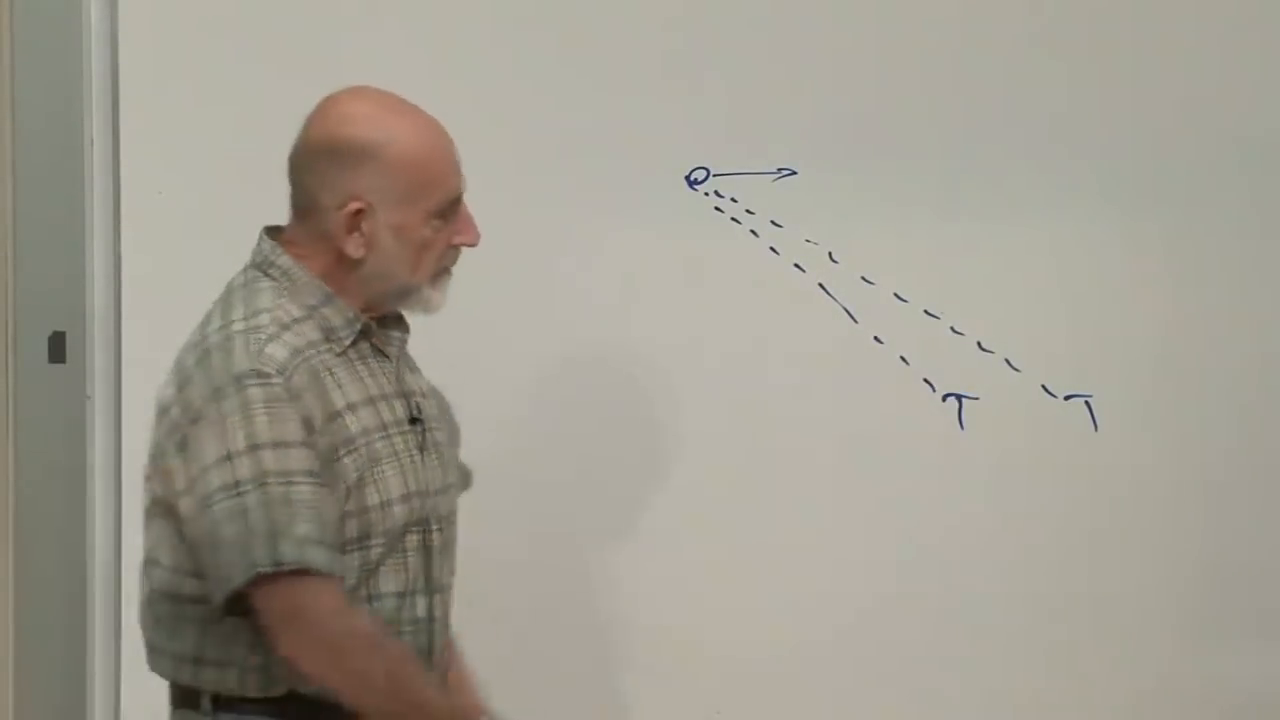
\includegraphics[width=0.78\textwidth]{lecture_05_figure_07.png}
  \caption{歴史的なニュートリノ測定の質問の際に議論された衛星座標系でのタイミングの概略。}
  \lectureframe{00:06:30}
\end{figure}

タイミングの議論は以下の力学には必要ない。それでもなお、もっともらしい桁の見積もりは確立した実験的説明と同じではないという注意として役に立つ。

\section{能動的対称性と系の選択}

先の議論であまりに曖昧なまま残された点に戻ろう。対称性とは正確には何か。直線上の粒子と次の指示を考える。
\begin{equation}
  x\longrightarrow x+1.
  \label{eq:l5-shift-one}
\end{equation}
これを理解する方法は二つある。\emph{受動的}変換は直線の点に付けられたラベルを付け替える。かつて\(x=0\)と呼ばれていた点は今や\(x'=1\)と呼ばれるかもしれないが、粒子は動いていない。\emph{能動的}変換はラベルを固定したまま粒子自体を\(x\)から\(x+1\)へ動かす。外部ポテンシャルに対するその位置を変えるのは二番目の操作だけである。

\begin{figure}[htbp]
  \centering
  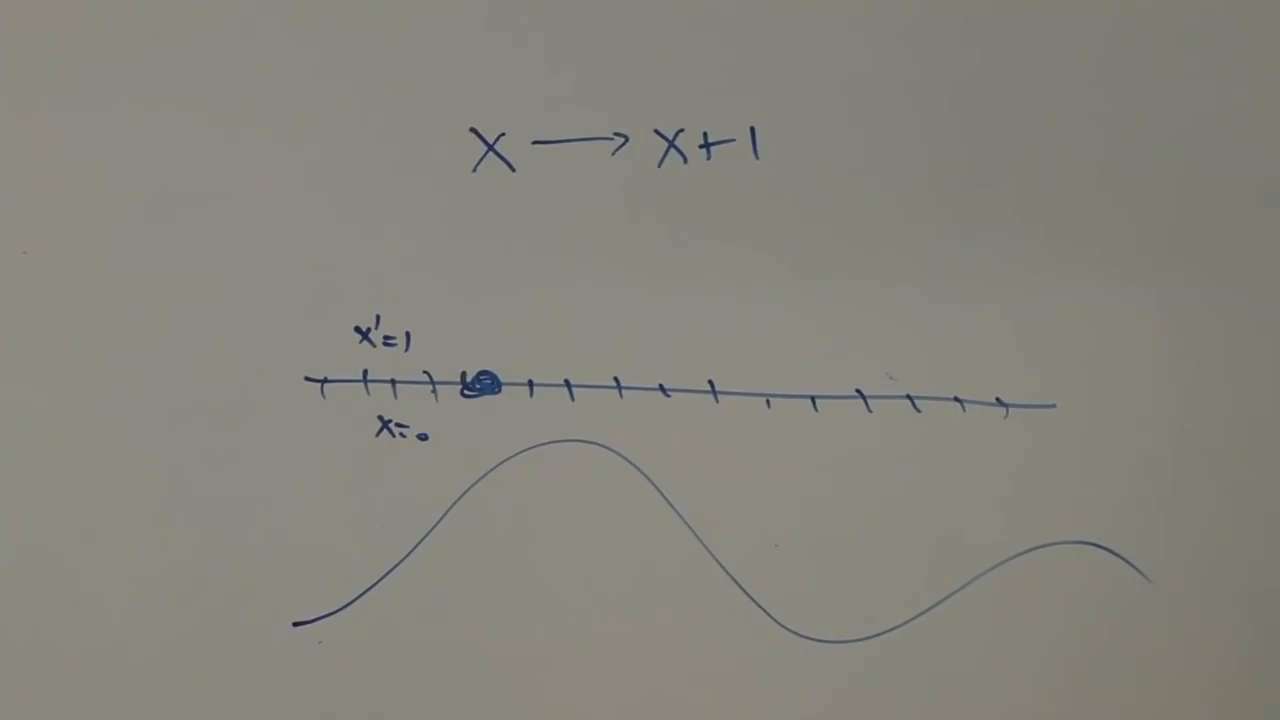
\includegraphics[width=0.82\textwidth]{lecture_05_figure_08.png}
  \caption{規則\(x\mapsto x+1\)、固定された座標線、および外部ポテンシャルが、能動的な運動を受動的なラベルの付け替えから区別する。}
  \lectureframe{00:11:20}
\end{figure}

\begin{classroomqa}
  \audiencequestion{粒子を動かすとそのポテンシャルエネルギーが変わるなら、そのポテンシャルの源は系から除外されているのですか。
  \lecturetimestamp{00:12:19--00:14:18}}
  \lecturerresponse{そのとおり。系を``ポテンシャル中の粒子''と呼ぶことは、世界を粒子と、\(V(x)\)を生み出す地球のような重い環境に分ける。地球も実際に反跳するが、その巨大な質量のためにこの近似ではその反跳は無視できる。固定された地球に対して粒子を動かすと\(V\)は変わりうるが、粒子と地球を一緒に並進させても変わらないであろう。}
\end{classroomqa}

\begin{classroomqa}
  \audiencequestion{先の回転の例では、位置だけでなく速度も変わりましたか。
  \lecturetimestamp{00:14:26--00:15:29}}
  \lecturerresponse{はい。剛体的な能動的回転は、ある瞬間の位置だけではなく履歴全体に作用する。位置と速度ベクトルの両方が回転される。対照的に、各時刻に適用される一定の並進は\(x\)を変えるが\(\dot x\)は変えないままにする。}
\end{classroomqa}

系と環境の区別は二度にわたって再び現れる。時間依存の装置が部分系とエネルギーを交換するとき、そして巨視的な摩擦が観測されない微視的運動の中にエネルギーを隠すときである。

\section{配置空間における無限小運動}

一般の力学系の配置とは、一般化座標\(q_i\)の空間における一点である。能動的な無限小変換は、可能なあらゆる配置を近傍の配置へと移す。我々は
\begin{equation}
  \delta q_i=\epsilon f_i(q),
  \label{eq:l5-general-transformation}
\end{equation}
と書く。ここで関数\(f_i\)は配置空間上の一つの固定された変位場を指定する。それらはすべての座標に依存してもよく、また消えるものがあってもよい。共通因子\(\epsilon\)は小さく、変換の形から歩みの大きさを分離する。

\begin{figure}[htbp]
  \centering
  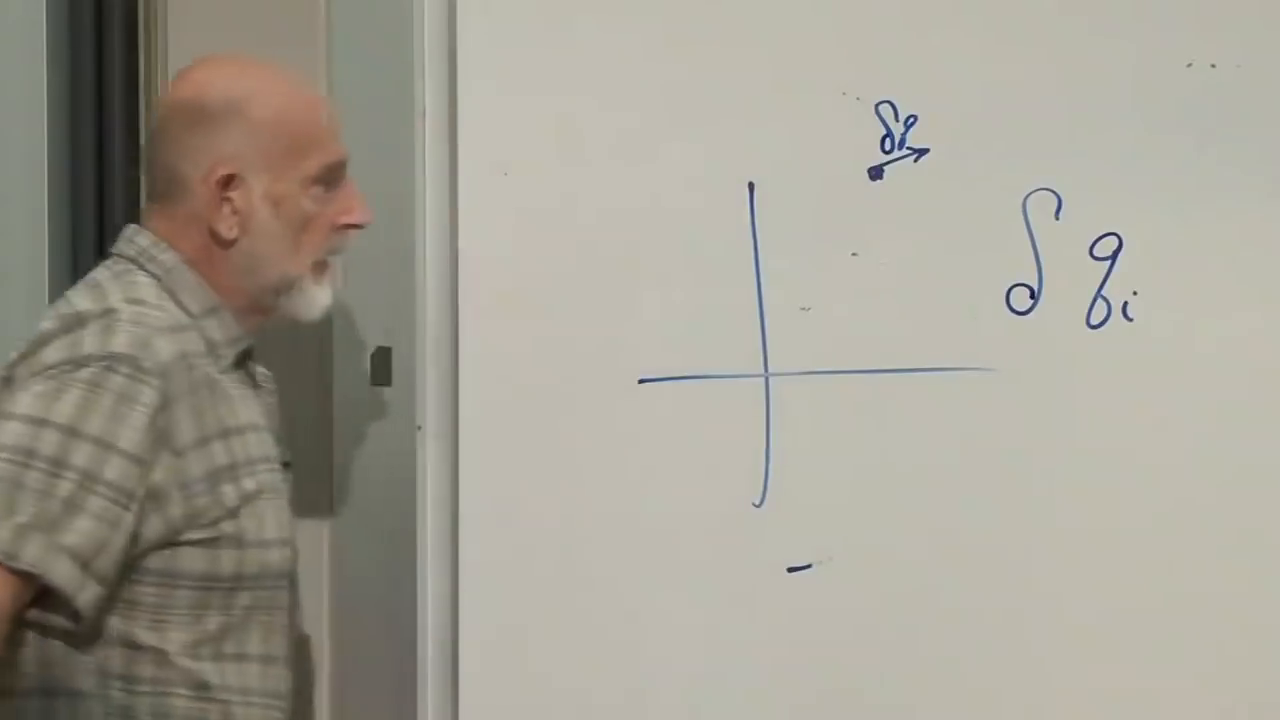
\includegraphics[width=0.75\textwidth]{lecture_05_figure_09.png}
  \caption{配置空間の各点に付随する変位ベクトル。}
  \lectureframe{00:16:50}
\end{figure}

\begin{figure}[htbp]
  \centering
  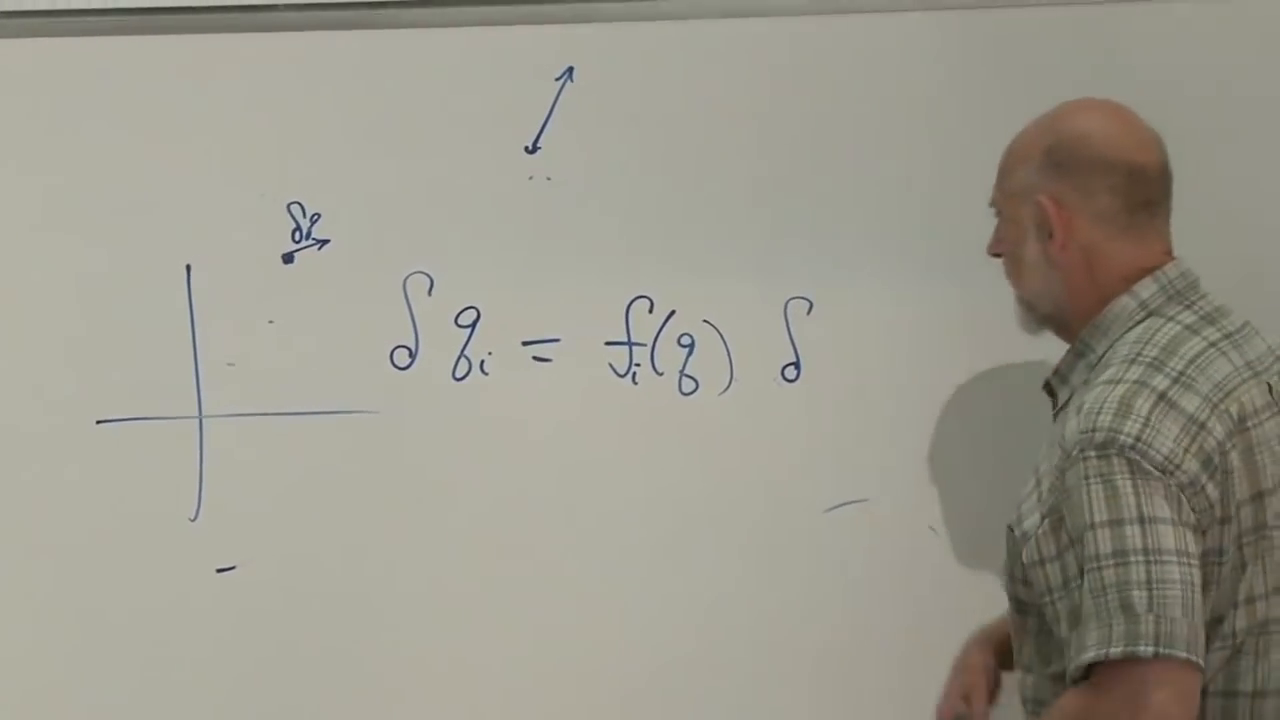
\includegraphics[width=0.80\textwidth]{lecture_05_figure_10.png}
  \caption{座標に依存する無限小変換
  \(\delta q_i=\epsilon f_i(q)\)。}
  \lectureframe{00:18:00}
\end{figure}

規則そのものには陽な時間依存性がない。したがって速度への作用は
\begin{equation}
  \delta\dot q_i=\frac{d}{dt}(\delta q_i)
  =\epsilon\sum_j\frac{\partial f_i}{\partial q_j}\dot q_j.
  \label{eq:l5-velocity-variation}
\end{equation}
である。並進の場合、\(f_x=1\)であるから\(\delta\dot x=0\)となる。回転の場合、\(f_i\)は位置に依存し、速度は変化する。

\begin{classroomqa}
  \audiencequestion{
  \(\delta q_i=\epsilon f_i(q)\)における最後の小さな因子は、どの点でも同じ定数か。
  \lecturetimestamp{00:19:58--00:20:51}}
  \lecturerresponse{はい。単一の定数\(\epsilon\)は、すべての座標変化を同じ小さな量について一次にするための帳簿上の仕掛けである。空間依存性を含むのは\(\epsilon\)ではなく関数\(f_i(q)\)であり、それら自身は小さくある必要はない。}
\end{classroomqa}

\section{何が変換を対称性にするのか}

能動的変換は一般にポテンシャルエネルギーを変化させる。それは運動エネルギーも変化させうる。曲線座標では運動項は
\begin{equation}
  T=\frac12\sum_{i,j}g_{ij}(q)\dot q_i\dot q_j,
  \label{eq:l5-kinetic-metric}
\end{equation}
の形をとるので、配置空間内を動くことによってその係数が変化しうる。極座標におけるおなじみの\(r^2\dot\theta^2\)項が最も単純な例である。

ここで変換が対称性であるとは、\emph{ラグランジアン全体}が一次の変化を持たないこと、すなわち
\begin{equation}
  \delta L=O(\epsilon^2),
  \label{eq:l5-symmetry-condition}
\end{equation}
であり、これは配置空間のあらゆる点で成り立たなければならず、ある特定の解が占める配置においてのみ成り立てばよいのではない。

例えば、\(x\mapsto x+\epsilon\)の下で
\begin{equation}
  \delta V=\frac{\partial V}{\partial x}\epsilon.
  \label{eq:l5-potential-variation}
\end{equation}
である。これが可能なあらゆる\(x\)に対して消えるならば、\(\partial V/\partial x=0\)、すなわちポテンシャルは\(x\)に依存しない。あらゆる空間方向への並進の下で不変ならば、それは定数である。

\begin{figure}[htbp]
  \centering
  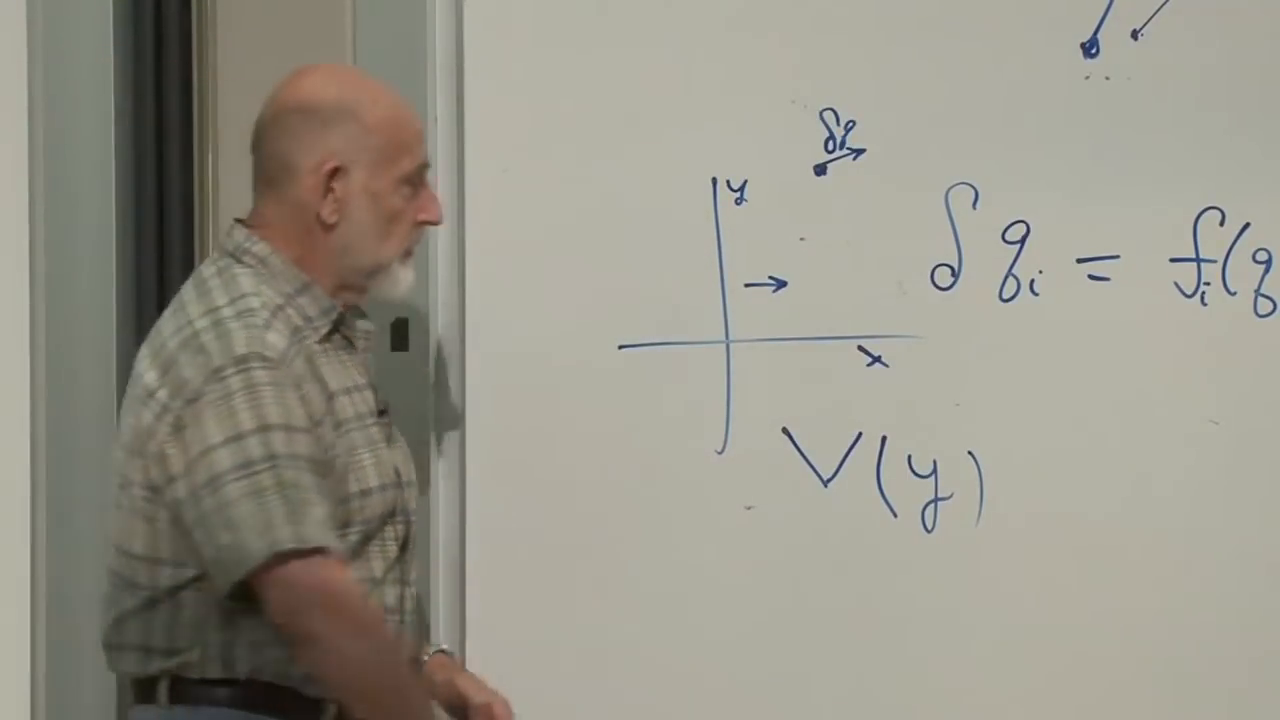
\includegraphics[width=0.80\textwidth]{lecture_05_figure_11.png}
  \caption{\(x\)に依存しないポテンシャル\(V(y)\)に対して試された\(x\)並進。}
  \lectureframe{00:23:40}
\end{figure}

滑らかな一径数族に対しては、あらゆる点で一次の変化が消えることにより、無限小の歩みを合成して有限の対称性とすることができる。

\begin{classroomqa}
  \audiencequestion{運動エネルギーとポテンシャルエネルギーは別々に不変でなければならないのか。
  \lecturetimestamp{00:24:44--00:25:33}}
  \lecturerresponse{いいえ。不変でなければならないのは全ラグランジアンのみである。座標--速度の混合項を含むラグランジアンもあり、そのようなものは\(T\)と\(V\)への有用な分離を許さないので、別々の不変性は意味のある問いですらないかもしれない。}
\end{classroomqa}

\begin{classroomqa}
  \audiencequestion{``変化なし''とは、厳密に変化がないことか、それとも無視できるほど小さい変化にすぎないことか。
  \lecturetimestamp{00:25:34--00:28:59}}
  \lecturerresponse{無限小変換に対しては、\(\epsilon\)に比例する項がないことを意味する。\(\epsilon^2\)の次数の項は局所計算では捨てられる。一次の条件が一径数軌道に沿ってどこでも成り立つので、局所的な歩みを繰り返せば有限の不変性が得られる。}
\end{classroomqa}

\section{運動量と角運動量の再導出}

ここで考察する厳密で時間に依存しない点対称性に対して、以前に証明された結果は
\begin{equation}
  Q=\sum_i p_i f_i(q),
  \qquad
  p_i=\frac{\partial L}{\partial\dot q_i},
  \qquad
  \dot Q=0.
  \label{eq:l5-noether-charge}
\end{equation}
である。因子\(\epsilon\)は\(Q\)に属するものではない。それは対称性の軌道に沿ってどれだけ進むかを測るだけである。

\begin{figure}[htbp]
  \centering
  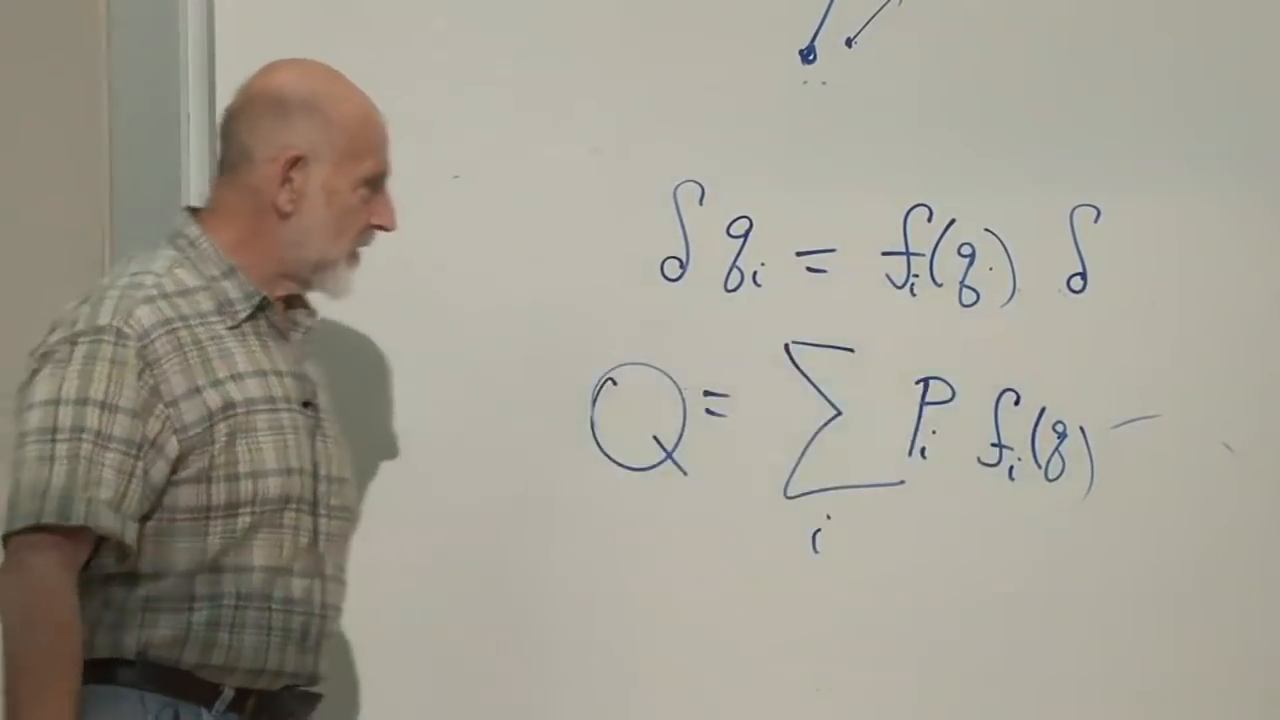
\includegraphics[width=0.82\textwidth]{lecture_05_figure_12.png}
  \caption{一般的な無限小変位とその保存ネーター電荷。}
  \lectureframe{00:30:00}
\end{figure}

\(x\)における並進に対して、\(f_x=1\)であり、\(Q=p_x\)である。完全な並進不変性は運動量の三成分すべての保存を与える。多数の相互作用する粒子に対しては、対称性はすべての粒子を一緒に並進させるので、相互作用が相対位置のみに依存するとき
\begin{equation}
  \mathbf P=\sum_a\mathbf p_a
  \label{eq:l5-total-momentum}
\end{equation}
が保存される。一つの粒子を残りに対して相対的に動かすことはこの対称性ではない。

\begin{figure}[htbp]
  \centering
  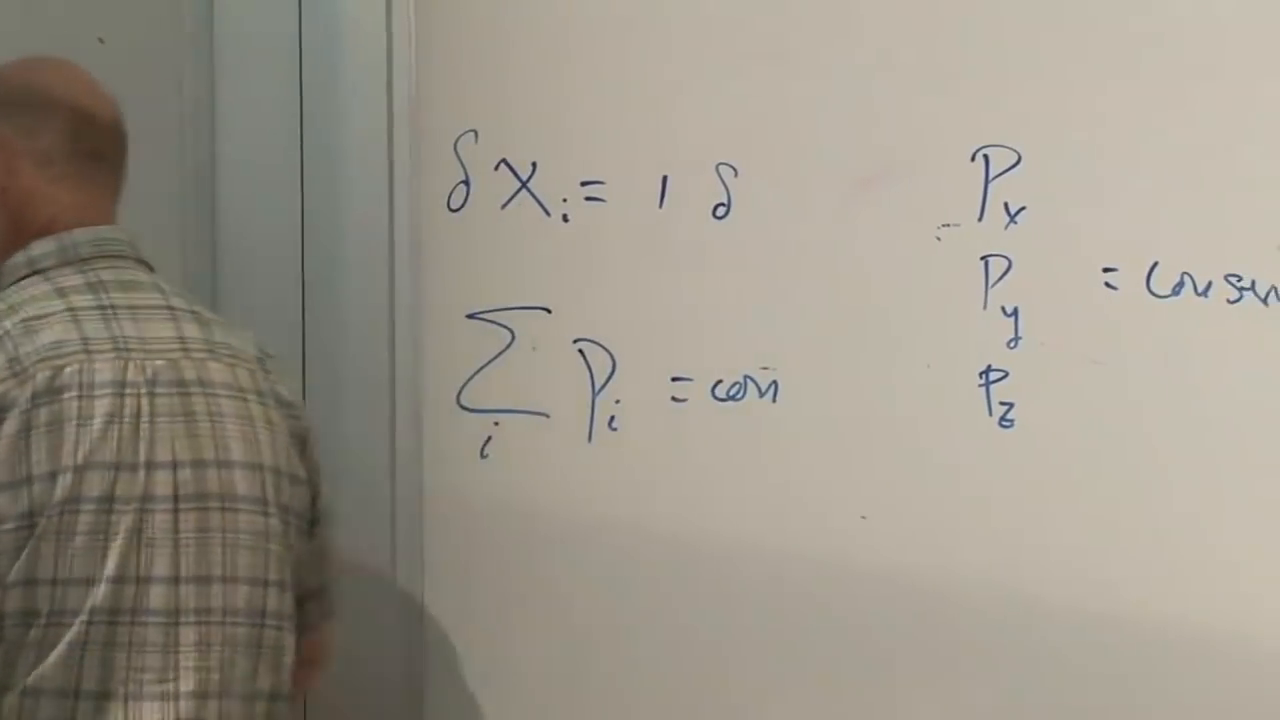
\includegraphics[width=0.80\textwidth]{lecture_05_figure_13.png}
  \caption{共通の並進は全運動量の成分ごとの保存を生じる。}
  \lectureframe{00:32:50}
\end{figure}

\(x\)-\(y\) 面内の無限小回転に対して、向きを
\begin{equation}
  \delta x=-y\epsilon,
  \qquad
  \delta y=x\epsilon.
  \label{eq:l5-planar-rotation}
\end{equation}
と選ぶ。これは半径を保存する。なぜなら
\begin{equation}
  \delta(x^2+y^2)
  =2x\delta x+2y\delta y=0.
  \label{eq:l5-radius-invariance}
\end{equation}

\begin{figure}[htbp]
  \centering
  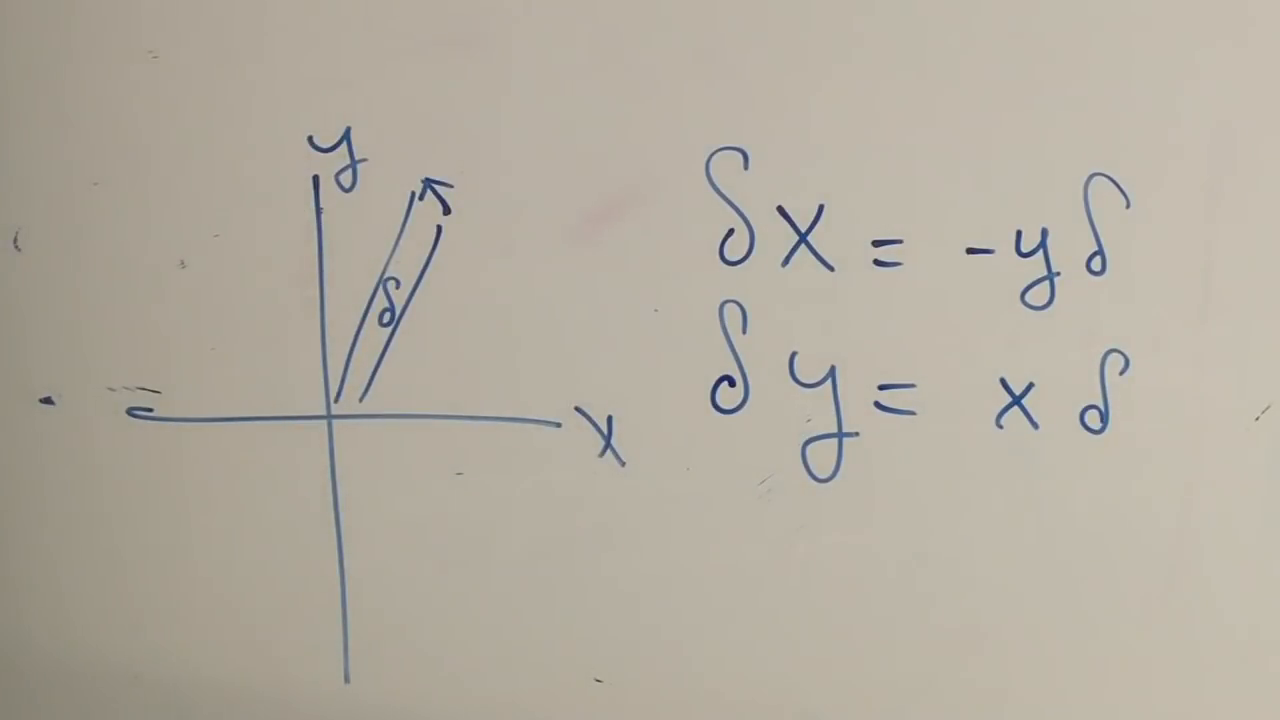
\includegraphics[width=0.76\textwidth]{lecture_05_figure_14.png}
  \caption{無限小平面回転の幾何と座標公式。}
  \lectureframe{00:35:05}
\end{figure}

式~\eqref{eq:l5-planar-rotation}を微分すると速度も同様に回転する。したがって \(\dot x^2+\dot y^2\) は不変であり、中心ポテンシャル \(V(\sqrt{x^2+y^2})\) は完全なラグランジアンを変えない。電荷は
\begin{equation}
  Q=-yp_x+xp_y=(\mathbf r\times\mathbf p)_z.
  \label{eq:l5-angular-charge}
\end{equation}

\begin{figure}[htbp]
  \centering
  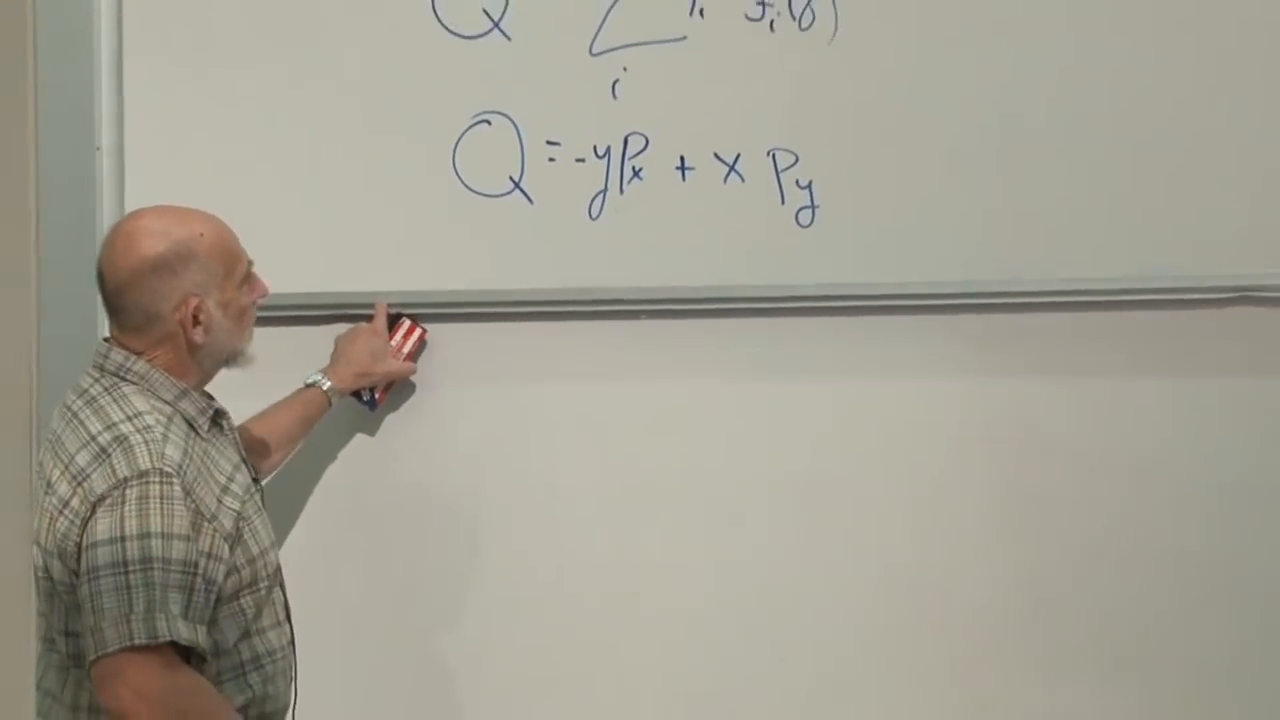
\includegraphics[width=0.76\textwidth]{lecture_05_figure_15.png}
  \caption{回転のネーター電荷、角運動量の \(z\) 成分。}
  \lectureframe{00:38:50}
\end{figure}

他の座標面内の回転は残りの成分を与える。多粒子の場合、保存されるベクトルは
\begin{equation}
  \mathbf J=\sum_a\mathbf r_a\times\mathbf p_a.
  \label{eq:l5-total-angular-momentum}
\end{equation}
中心恒星ポテンシャル中の惑星が基本例である。すべての回転の下での不変性は角運動量のすべての成分の保存を意味する。

\begin{classroomqa}
  \audiencequestion{一方からの微分と他方からの微分が異なる鋭いカスプでは何が起こるか。
  \lecturetimestamp{00:42:25--00:44:21}}
  \lecturerresponse{それは正当な限定である。現在の議論は一意な微分をもつ微分可能な関数を仮定している。滑らかな極大で釣り合った物体のような不安定平衡はそれ自体問題ではない。そこでは微分が存在し消えるからである。文字通りのカスプには修正された取り扱いが必要である。}
\end{classroomqa}

\begin{classroomqa}
  \audiencequestion{変換パラメータが時間に依存しないなら、なぜ回転は速度を変えるのか。
  \lecturetimestamp{00:44:23--00:45:23}}
  \lecturerresponse{パラメータは一定であるが、変位場は座標に依存する。普遍的な規則は
  \(\delta\dot q_i=d(\delta q_i)/dt\) である。並進は \(\delta x\) が一定であり、一方、回転は \(\delta x=-y\epsilon\) をもち、したがって
  \(\delta\dot x=-\dot y\epsilon\) となる。}
\end{classroomqa}

\section{初等的な運動エネルギー引くポテンシャル形を超えて}

磁場のない通常の非相対論的粒子に対するデカルト座標では \(L=T-V\) である。より一般の座標は式~\eqref{eq:l5-kinetic-metric}の二次形式を生む。磁場は速度に線形な項を導入し、概略 \(\mathbf A(q)\cdot\dot{\mathbf q}\) であり、座標と速度を混ぜる。そのような場合、\(L(q,\dot q,t)\) を一つの関数として扱う方が、すべての項を従来の運動エネルギーとポテンシャルの枠に押し込むよりよい。

\begin{figure}[htbp]
  \centering
  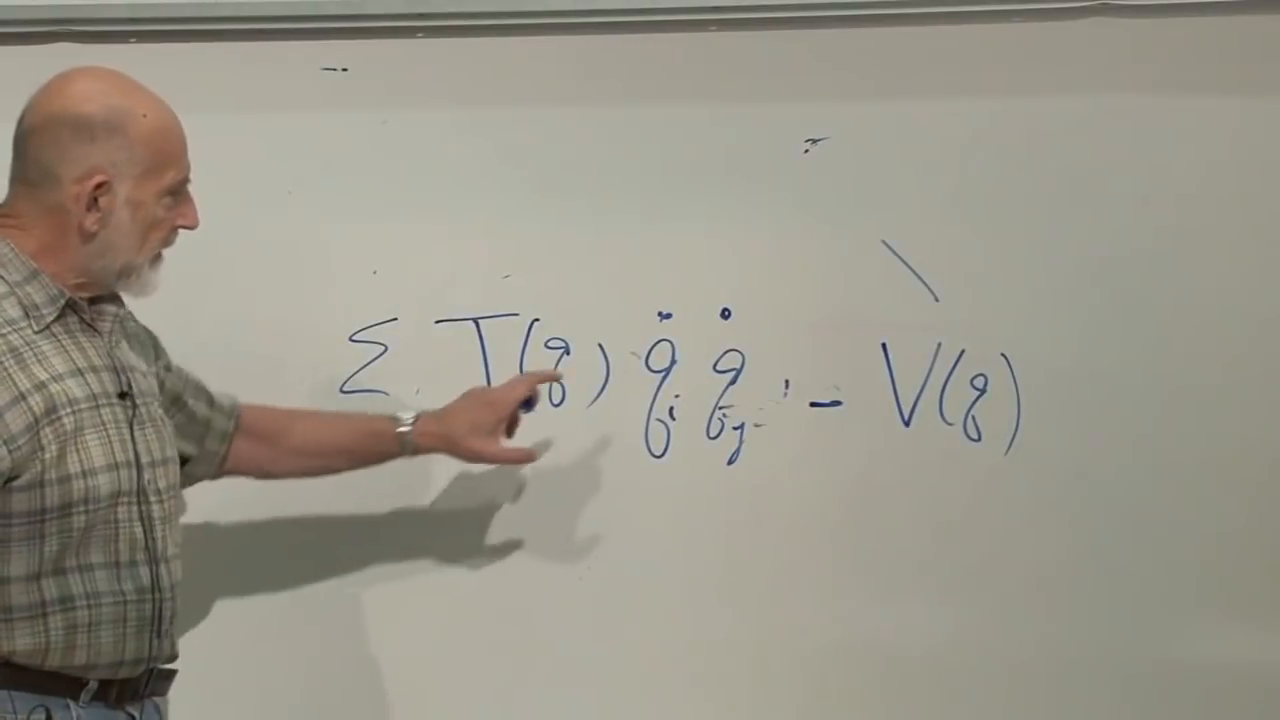
\includegraphics[width=0.80\textwidth]{lecture_05_figure_16.png}
  \caption{座標に依存する一般の二次の運動項と座標のみのポテンシャル。}
  \lectureframe{00:47:20}
\end{figure}

\begin{classroomqa}
  \audiencequestion{なぜラグランジアンは運動エネルギーとポテンシャルエネルギーにきれいに分離できないことがあるのか、そしてそれは依然として \(T-V\) と定義されるのか。
  \lecturetimestamp{00:45:26--00:48:13}}
  \lecturerresponse{障害は曲線座標から、あるいは磁気のような真に速度に依存する相互作用から来るかもしれない。ラグランジアンが二次の速度形式から座標のみの関数を引いたものからなるときにのみ、それらの部分を \(T\) と \(V\) と呼ぶ。そうでなければラグランジアンは \(q\) と \(\dot q\) の完全に良い関数であり続けるが、その分割は有益ではない。エネルギーの正しい一般的定義はハミルトニアンから来る。}
\end{classroomqa}

\begin{classroomqa}
  \audiencequestion{最初の講義の鎖の例は最小作用の応用だったのか。
  \lecturetimestamp{00:48:15--00:49:45}}
  \lecturerresponse{それは最小エネルギーに支配される平衡問題であり、停留作用によって選ばれた履歴ではない。通常の \(T-V\) 系の静的解では \(\dot p_i=0\) であり、オイラー--ラグランジュ方程式は \(\partial V/\partial q_i=0\) に帰着する。これはポテンシャルの停留点の条件である。}
\end{classroomqa}

運動量と角運動量は今や空間対称性に結びつけられた。目立って欠けている量はエネルギーである。

\section{時間並進不変性}

\(t_0\) に始まり \(t_1\) に終わり、結果を生む実験を想像せよ。同じ準備を後で繰り返し、\(t_0+\Delta t\) に始まり \(t_1+\Delta t\) に終わる。結果が変わらなければ、系は時間における能動的並進の下で不変である。

\begin{figure}[htbp]
  \centering
  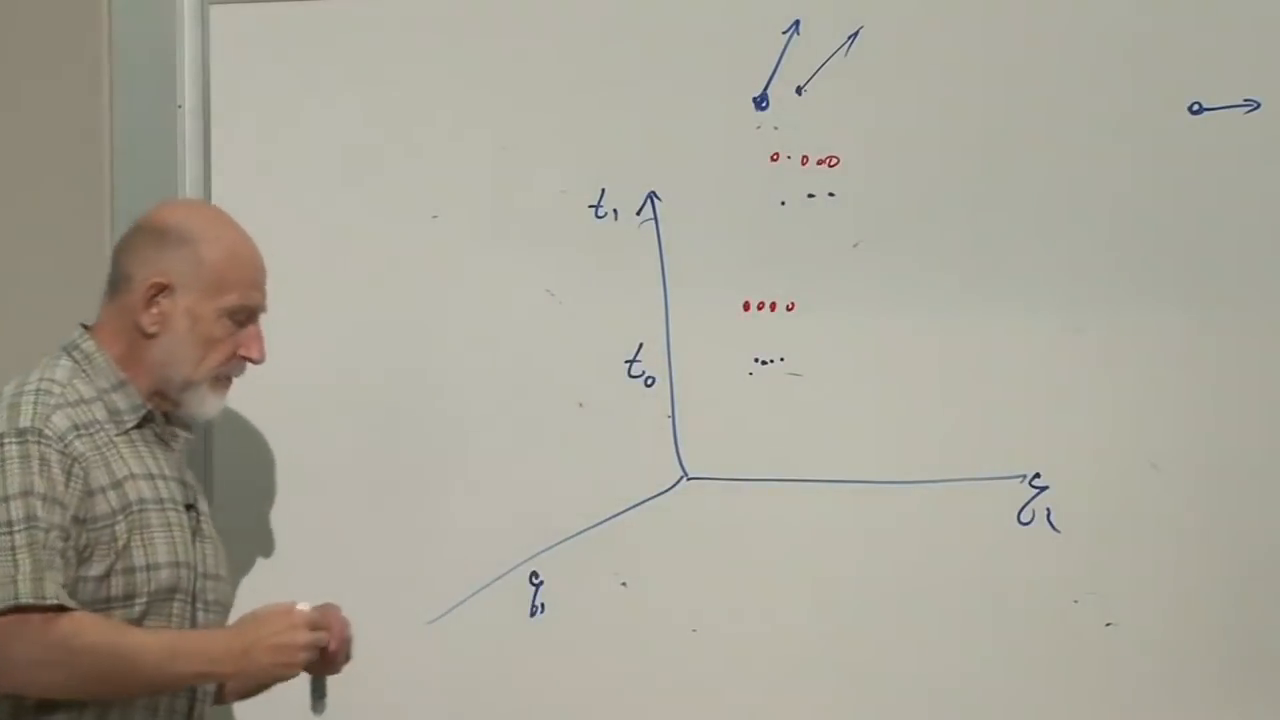
\includegraphics[width=0.82\textwidth]{lecture_05_figure_17.png}
  \caption{配置空間の履歴における実験とその時間並進されたコピー。}
  \lectureframe{00:52:45}
\end{figure}

コンデンサー板間の荷電粒子はこの対称性の破れを例示する。板の電荷が固定されていれば、同じ実験をいつでも行える。外部発電機が板を定常的に充電しているなら、粒子はいつ放出されるかに応じて異なる電場を見る。そのとき粒子は明示的に駆動された部分系である。

\begin{figure}[htbp]
  \centering
  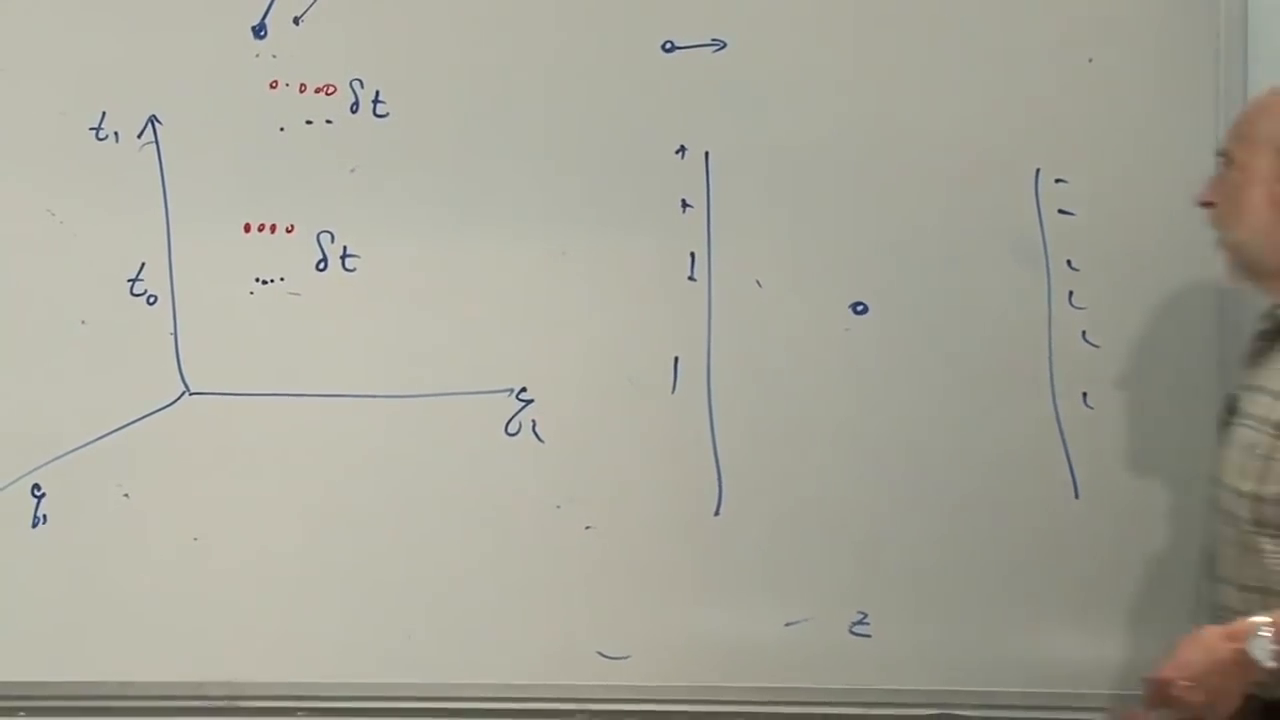
\includegraphics[width=0.82\textwidth]{lecture_05_figure_18.png}
  \caption{固定されたコンデンサー板と外部から変化するコンデンサー板を時間並進図の隣に対比。}
  \lectureframe{00:54:45}
\end{figure}

同じ点は振動子にも現れる。
\begin{equation}
  L=\frac12m\dot x^2-\frac12k(t)x^2.
  \label{eq:l5-driven-oscillator}
\end{equation}
外部の電場または磁場は、物質をゆっくり変化させ、したがってその有効ばね定数を変化させうる。\(k\)が変化するならば、振動子の実験を時間的にずらすと結果が変わる。

\begin{figure}[htbp]
  \centering
  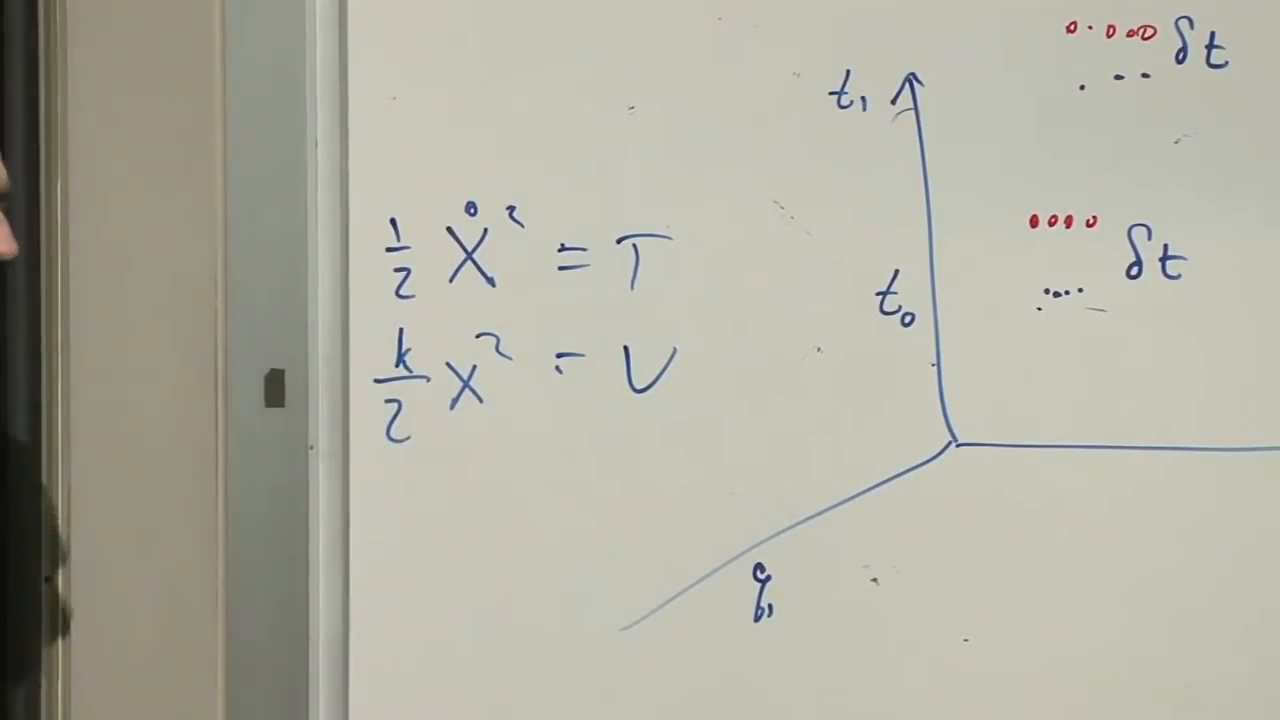
\includegraphics[width=0.78\textwidth]{lecture_05_figure_19.png}
  \caption{時間依存のばね定数を議論している間の振動子の運動エネルギー項とポテンシャル項。}
  \lectureframe{00:56:45}
\end{figure}

\(k\)を変化させる装置を系に含めるならば、完全な閉じた実験は再び時間並進でき、その全エネルギーは保存される。見かけの非保存は、我々が選んだ境界を越えたエネルギーの交換である。

休憩中に、小さな変換パラメータは\(\epsilon\)と改名され、視覚的に紛らわしい表式\(\delta x=\delta\)を避けた。エミー・ネーターに関する本のクラス推薦も、共有読書リストのために記録された。

\begin{classroomqa}
  \audiencequestion{ラグランジアンが\(T-V\)として与えられないならば、それはどこから来るのか。
  \lecturetimestamp{01:00:17--01:02:24}}
  \lecturerresponse{それは実験から推論され、既知の運動方程式から再構成され、対称性やその他の理論的原理から推測され、あるいは試行錯誤によって見出されうる。ひとたび\(L(q,\dot q,t)\)が与えられれば、オイラー--ラグランジュの計算がそれを運動方程式に変える。形式的な議論は、その起源をまず決着させることを我々に要求しない。}
\end{classroomqa}

時間並進不変性の操作的判定は、いまや即座に得られる。\(q\)と\(\dot q\)の知識が、時計の時刻をも知ることなしに\(L\)を決定するのに十分であるならば、
\begin{equation}
  \frac{\partial L}{\partial t}=0.
  \label{eq:l5-no-explicit-time}
\end{equation}
これは、\(L(q(t),\dot q(t))\)が運動に沿って一定であると言っているのではない。それは、発展する座標と速度が担う以上の時間依存性が存在しないと言っているだけである。

回転する重いダンベルは、もう一つの駆動された例を与える。その規定された運動が、軽い試験粒子に対して時間変化する重力ポテンシャルを生み出すならば、試験粒子のラグランジアンは陽に時間に依存する。代わりにダンベルを力学的に扱えば、系は拡大され、その外部時間依存性は取り除かれる。

\begin{figure}[htbp]
  \centering
  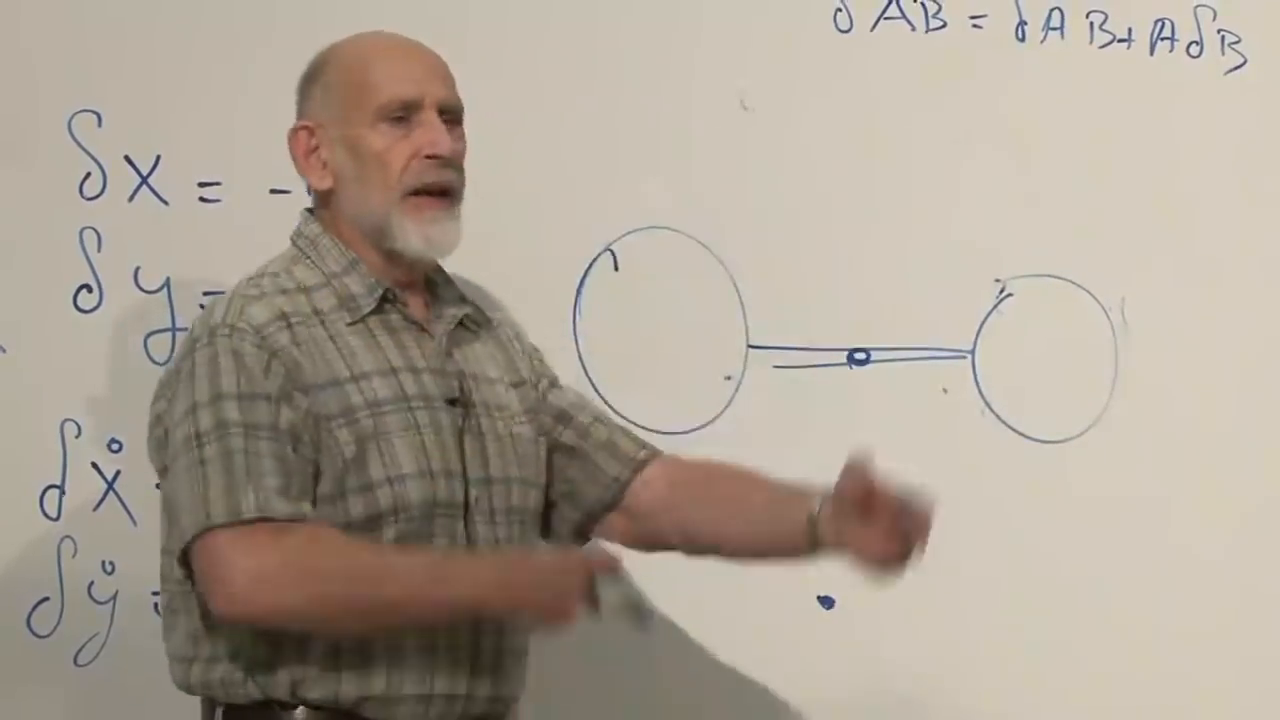
\includegraphics[width=0.80\textwidth]{lecture_05_figure_20.png}
  \caption{規定された回転ダンベルは、より軽い粒子に対する時間依存の外部源として働く。}
  \lectureframe{01:06:25}
\end{figure}

\section{ハミルトニアンの導出}

エネルギーの公式を知らず、おそらくラグランジアン自体が保存されるのではないかと推測したとしよう。直接的な判定は、実際の軌道に沿ってそれを微分することである。簡単のため、まず陽な時間依存性がない場合から始める。
\begin{equation}
  \frac{dL}{dt}
  =\sum_i\left(
    \frac{\partial L}{\partial q_i}\dot q_i
    +\frac{\partial L}{\partial\dot q_i}\ddot q_i
  \right).
  \label{eq:l5-chain-rule-no-time}
\end{equation}

\begin{figure}[htbp]
  \centering
  \includegraphics[width=0.72\textwidth]{lecture_05_figure_02.png}
  \caption{軌道に沿った\(L(q_i,\dot q_i)\)の微分を始める。}
  \lectureframe{01:08:51}
\end{figure}

\begin{classroomqa}
  \audiencequestion{連鎖律の表式に和が欠けていないか。
  \lecturetimestamp{01:10:39--01:11:05}}
  \lecturerresponse{はい。すべての座標とすべての速度がラグランジアンを変えうるので、両方の項は\(i\)について和をとる。}
\end{classroomqa}

正準運動量とオイラー--ラグランジュ方程式を用いると、
\begin{equation}
  p_i=\frac{\partial L}{\partial\dot q_i},
  \qquad
  \dot p_i=\frac{\partial L}{\partial q_i}.
  \label{eq:l5-p-and-pdot}
\end{equation}
そのとき式~\eqref{eq:l5-chain-rule-no-time}は次になる。
\begin{align}
  \frac{dL}{dt}
  &=\sum_i(\dot p_i\dot q_i+p_i\ddot q_i)
  \notag\\
  &=\frac{d}{dt}\sum_i p_i\dot q_i.
  \label{eq:l5-product-rule}
\end{align}
``魔法''は積の法則にすぎない。

\begin{figure}[htbp]
  \centering
  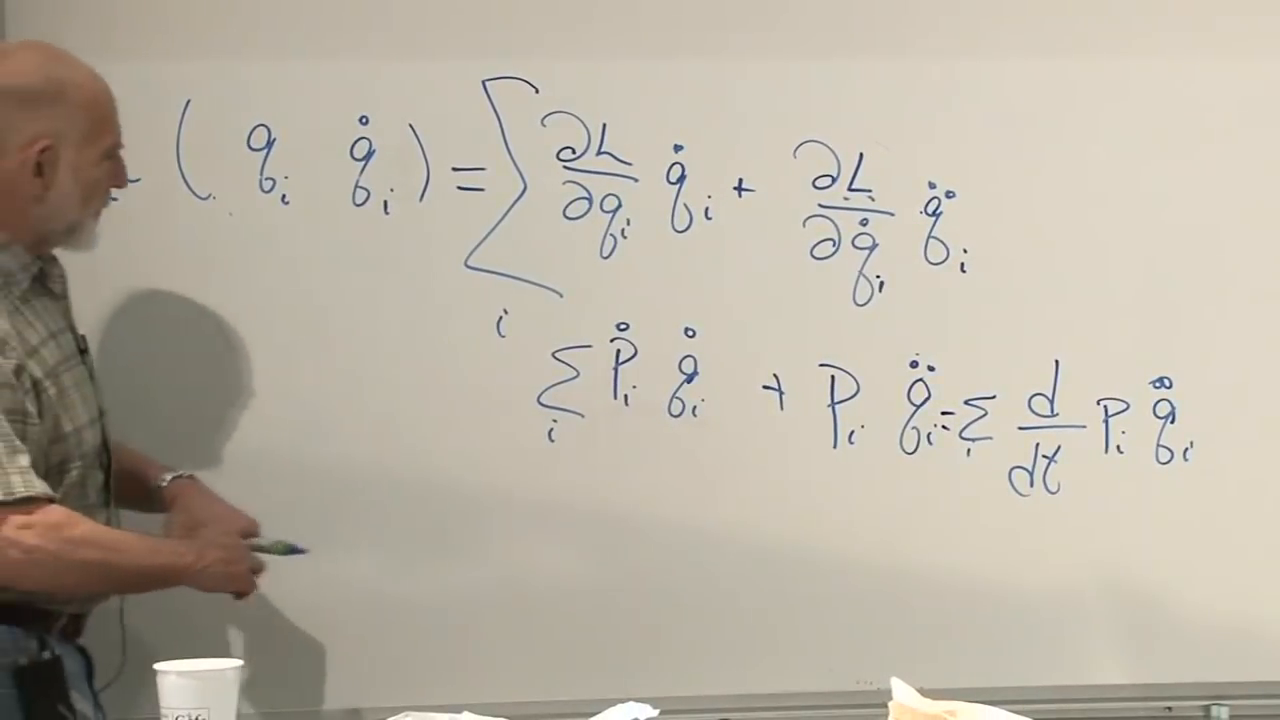
\includegraphics[width=0.84\textwidth]{lecture_05_figure_21.png}
  \caption{連鎖律は、運動方程式を用いて、\(\sum_i p_i\dot q_i\)の微分に変換された。}
  \lectureframe{01:13:45}
\end{figure}

\begin{classroomqa}
  \audiencequestion{積の中の最後の\(q_i\)はドット一つか、それとも二つか。
  \lecturetimestamp{01:14:31--01:15:32}}
  \lecturerresponse{積の内部では\(p_i\dot q_i\)であり、ドットは一つである。積を微分すると
  \(\dot p_i\dot q_i+p_i\ddot q_i\)となり、これが展開された第二項の二つのドットを説明する。}
\end{classroomqa}

二つの微分を引くと保存する組み合わせが得られる。歴史的な慣習はその負を選び、それをハミルトニアンと呼ぶ。
\begin{equation}
  H=\sum_i p_i\dot q_i-L.
  \label{eq:l5-hamiltonian-definition}
\end{equation}

\begin{figure}[htbp]
  \centering
  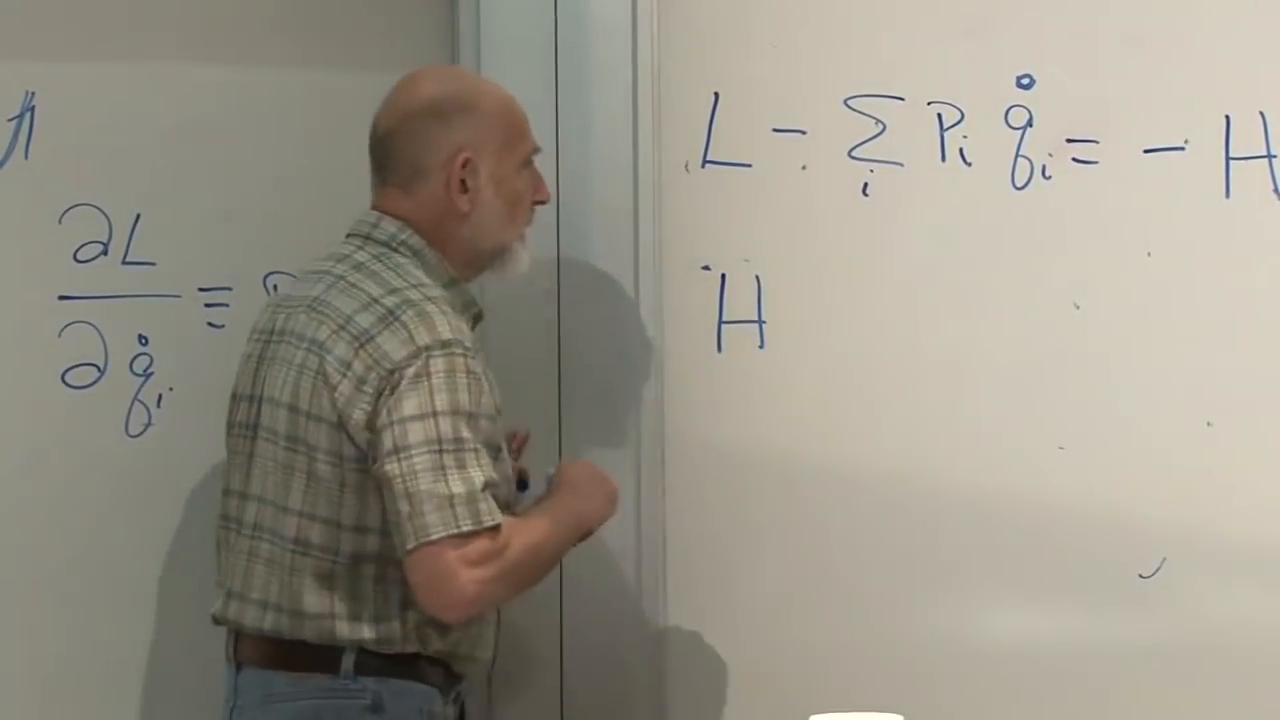
\includegraphics[width=0.80\textwidth]{lecture_05_figure_22.png}
  \caption{保存する組み合わせ\(L-\sum_i p_i\dot q_i=-H\)とハミルトニアンの定義。}
  \lectureframe{01:18:05}
\end{figure}

ポテンシャル中の一粒子に対して、
\begin{equation}
  L=\frac12m\dot x^2-V(x),
  \qquad p=m\dot x.
  \label{eq:l5-particle-lagrangian}
\end{equation}
したがって
\begin{align}
  H&=p\dot x-L
  \notag\\
   &=m\dot x^2-\left(\frac12m\dot x^2-V(x)\right)
  \notag\\
   &=\frac12m\dot x^2+V(x)=T+V.
  \label{eq:l5-particle-energy}
\end{align}

\begin{figure}[htbp]
  \centering
  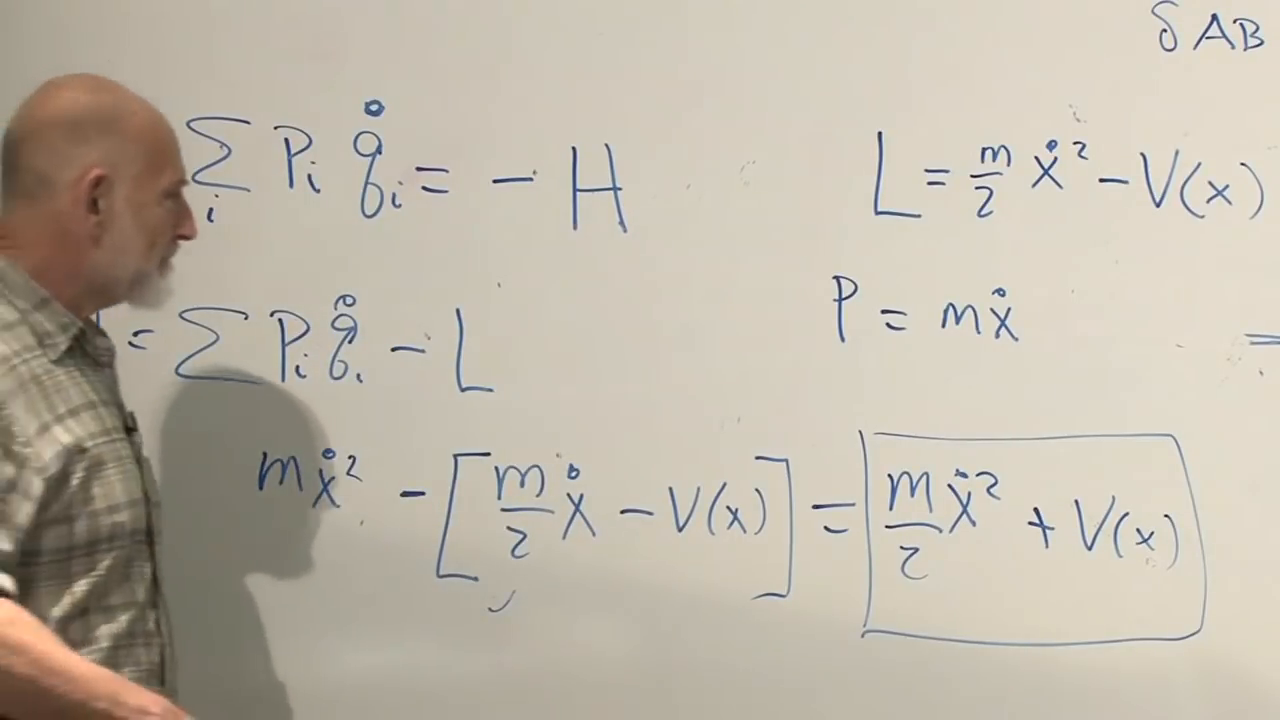
\includegraphics[width=0.86\textwidth]{lecture_05_figure_23.png}
  \caption{ポテンシャル中の粒子のハミルトニアンは、よく知られた運動エネルギーとポテンシャルエネルギーの和に帰着する。}
  \lectureframe{01:20:50}
\end{figure}

この導出は\(L\)の特定の形を仮定しなかった。したがって、\(T+V\)ではなく式~\eqref{eq:l5-hamiltonian-definition}が、この形式におけるエネルギーの一般的定義である。

\section{陽な時間依存性とエネルギーの交換}

連鎖律において陽な時間依存性を復元する。
\begin{equation}
  \frac{dL}{dt}
  =\sum_i\left(
    \frac{\partial L}{\partial q_i}\dot q_i
    +\frac{\partial L}{\partial\dot q_i}\ddot q_i
  \right)
  +\frac{\partial L}{\partial t}.
  \label{eq:l5-full-chain-rule}
\end{equation}
左辺は運動に沿った全微分である。最後の偏微分は\(q\)と\(\dot q\)を固定し、外部で変化するパラメータのみを微分する。同じ積の法則の手順を繰り返すと次が得られる。
\begin{equation}
  \boxed{\frac{dH}{dt}=-\frac{\partial L}{\partial t}}.
  \label{eq:l5-hamiltonian-time}
\end{equation}

\begin{figure}[htbp]
  \centering
  \includegraphics[width=0.70\textwidth]{lecture_05_figure_04.png}
  \caption{ハミルトニアンは、ラグランジアンが陽に時間に依存することを通じてのみ変化する。}
  \lectureframe{01:37:22}
\end{figure}

式~\eqref{eq:l5-driven-oscillator}の駆動振動子について、
\begin{equation}
  \frac{\partial L}{\partial t}
  =-\frac12\dot k(t)x^2,
  \qquad
  \dot H=\frac12\dot k(t)x^2.
  \label{eq:l5-driven-energy-rate}
\end{equation}
\(x=0\)では瞬間的な変化率は消える。原点から離れると、ばね定数を変えることは\(x^2\dot k\)に比例する割合で仕事をする。

\begin{classroomqa}
  \audiencequestion{エネルギーが保存されないなら、その定義はハミルトニアンの時間微分なのか。
  \lecturetimestamp{01:27:11--01:28:04}}
  \lecturerresponse{いいえ。エネルギーは\(H\)である。その導関数は、そのエネルギーがどのように変化するかを教えてくれる。ラグランジアンがよく知られた形をとるときは\(H=T+V\)であり、そうでないときは式~\eqref{eq:l5-hamiltonian-definition}が定義を与える。系を外部の駆動源を含むように拡大すれば、全ハミルトニアンの保存が回復する。}
\end{classroomqa}

\begin{classroomqa}
  \audiencequestion{これは、遠心力とコリオリの項が現れた、回転するメリーゴーラウンド上の先ほどの観測者にどのように当てはまるのか。
  \lecturetimestamp{01:28:08--01:29:52}}
  \lecturerresponse{定常的に回転する座標系は、時間に依存する変数変換であり、固定された空間的対称性でも、時間における単純な並進でもない。その変換されたラグランジアンを用いてハミルトニアンを構成することはできるが、その別個の計算は、磁気力を論じるまで延期するのが最善である。なぜなら、その代数は密接に関連する形をとるからである。}
\end{classroomqa}

\section{一目でわかるラグランジアンの道具箱}

全体の構造は今やコンパクトなまとまりとして書くことができる。
\begin{align}
  L&=L(q_i,\dot q_i,t),
  \notag\\
  p_i&=\frac{\partial L}{\partial\dot q_i},
  \qquad
  \dot p_i=\frac{\partial L}{\partial q_i},
  \notag\\
  \delta q_i&=\epsilon f_i(q)
  \quad\Longrightarrow\quad
  Q=\sum_i p_i f_i(q),\quad \dot Q=0,
  \notag\\
  H&=\sum_i p_i\dot q_i-L,
  \qquad
  \dot H=-\frac{\partial L}{\partial t}.
  \label{eq:l5-toolkit}
\end{align}

\begin{figure}[htbp]
  \centering
  \includegraphics[width=0.66\textwidth]{lecture_05_figure_03.png}
  \caption{板書の復習は\(L(q,\dot q,t)\)、正準運動量、そしてオイラー--ラグランジュ方程式から始まる。}
  \lectureframe{01:31:37}
\end{figure}

これらの公式には、定義、運動方程式、通常の連続対称性の電荷、そして時間並進の電荷が含まれている。技巧はほとんどない。重要なのは、無関係な式を暗記するのではなく、それらを再導出できることである。

\section{なぜラグランジアン力学やハミルトン力学を使うのか。}

\begin{classroomqa}
  \audiencequestion{力学は\(L\)でも\(H\)でも等しく記述できるのか、そしてなぜ一方の定式化を選ぶのか。
  \lecturetimestamp{01:37:16--01:39:18}}
  \lecturerresponse{ルジャンドル変換が正則であるとき、それらは等価であるが、異なる構造を強調する。ラグランジアンは停留作用から自然に始まる。ハミルトン力学は最初はより抽象的であるが、その方程式は単純であり、量子力学において中心的となる。ハミルトニアンはエネルギーであるが、その役割は保存則だけよりもはるかに大きい。}
\end{classroomqa}

\begin{classroomqa}
  \audiencequestion{ニュートンはエネルギーの保存のハミルトン形式を知っていたのか。
  \lecturetimestamp{01:39:29--01:39:56}}
  \lecturerresponse{歴史的記録が示す限り、この定式化では知らなかった。ニュートンが述べた枠組みは力の法則\(F=ma\)であった。}
\end{classroomqa}

\begin{classroomqa}
  \audiencequestion{なぜすべての物理系がラグランジアンを持たなければならないのか。それは単に実験的なことなのか。
  \lecturetimestamp{01:39:57--01:42:37}}
  \lecturerresponse{ここで扱う閉じた系については、それは経験的事実であり、またより深い量子論的記述からも従う。数学的に整合する微分方程式で、オイラー--ラグランジュ方程式ではないものを発明することはできる。例えば、\(\dot x=-x\)は完全に解けるが、基本的な閉じた一自由度の法則としては、散逸の情報を失う性格を持つ。古典力学は論理的に量子力学に先行するものではなく、その基本的構造は量子力学から受け継がれている。詳細な理由は後述する。}
\end{classroomqa}

\begin{classroomqa}
  \audiencequestion{すべての実在の閉じた系がラグランジアンを持つなら、ラグランジアンと呼ぶすべての関数が自然界に見出される系に対応するのか。
  \lecturetimestamp{01:42:39--01:42:54}}
  \lecturerresponse{いいえ。形式的な計算は、既知のいかなる物理系によっても実現されない多くの関数を許容する。}
\end{classroomqa}

\begin{classroomqa}
  \audiencequestion{ラグランジアンは主にポテンシャルを発明するための道具なのか。
  \lecturetimestamp{01:42:54--01:43:32}}
  \lecturerresponse{それはそれよりも広い。候補となる力学系を組織化することができ、運動方程式へのしばしば最短の実用的な道である。}
\end{classroomqa}

二重振り子はその実用的な利点を示している。二つの角度を選び、両方の質点の速度をそれらの角度とその時間導関数で表して計算し、\(T-V\)を形成し、オイラー--ラグランジュ方程式に拘束力を暗黙のうちに処理させる。これは、\(F=ma\)ですべての張力と加速度を分解するよりもかなり簡潔である。

\begin{figure}[htbp]
  \centering
  \includegraphics[width=0.84\textwidth]{lecture_05_figure_05.png}
  \caption{エネルギー変化率の恒等式は、二重振り子のスケッチのそばの板書に残っている。}
  \lectureframe{01:45:39}
\end{figure}

\begin{figure}[htbp]
  \centering
  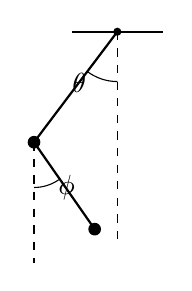
\begin{tikzpicture}[scale=1.15]
    \draw[thick] (-0.5,0) -- (0.5,0);
    \fill (0,0) circle (0.045);
    \draw[dashed] (0,0) -- (0,-2.3);
    \draw[thick] (0,0) -- (-0.92,-1.22);
    \fill (-0.92,-1.22) circle (0.07);
    \draw[dashed] (-0.92,-1.22) -- (-0.92,-2.55);
    \draw[thick] (-0.92,-1.22) -- (-0.25,-2.18);
    \fill (-0.25,-2.18) circle (0.07);
    \draw (0,-0.55) arc (-90:-127:0.55);
    \node at (-0.42,-0.56) {$\theta$};
    \draw (-0.92,-1.72) arc (-90:-55:0.48);
    \node at (-0.56,-1.72) {$\phi$};
  \end{tikzpicture}
  \caption{二重振り子の一般化角座標。}
\end{figure}

変数変換も同様に効率的である。すなわち、各々の力の方程式を別々に変換するのではなく、一つのラグランジアンを変換してからその方程式を導出するのである。

\begin{classroomqa}
  \audiencequestion{二重振り子は本質的に、太陽・地球・月のような別の三体問題であって、一つの物体を固定点として扱うものではないのか。
  \lecturetimestamp{01:45:06--01:45:25}}
  \lecturerresponse{その類推は階層構造を捉えているが、棒は異なる拘束を課す。いずれの場合でも、非常に質量の大きい、あるいは固定された構成要素は、近似において基準となる構造として扱うことができる。}
\end{classroomqa}

\begin{classroomqa}
  \audiencequestion{二重振り子は\(T-V\)を用いるが、より一般的なラグランジアンがちょうど強調されたところである。\(T-V\)はいつ妥当なのか。
  \lecturetimestamp{01:46:08--01:46:58}}
  \lecturerresponse{慣性系から見た通常の非相対論的粒子で、磁場による速度結合がない場合には、おなじみの形が当てはまる。回転系、相対論的系、磁場はより一般的な項を必要とする。}
\end{classroomqa}

\begin{classroomqa}
  \audiencequestion{衝突はこの記述の範囲外なのか。
  \lecturetimestamp{01:47:00--01:48:05}}
  \lecturerresponse{弾性衝突は短距離力に由来し、したがってポテンシャルに由来する。非弾性衝突は微視的レベルでは力学的にとどまるが、エネルギーは内部振動、変形、熱へと入っていく。それらの自由度を省いた重心記述は不完全である。}
\end{classroomqa}

\begin{classroomqa}
  \audiencequestion{バットで打たれた野球ボールを\(F=ma\)で解析できるか。
  \lecturetimestamp{01:48:05--01:48:33}}
  \lecturerresponse{粗いレベルでのみ可能である。完全な記述は、変形、発熱、ボールの損傷の可能性、そしておそらくバットの折損まで追わなければならない。それらの内部自由度があるために、現実的な衝突は質点の衝突よりはるかに難しいのである。}
\end{classroomqa}

\begin{classroomqa}
  \audiencequestion{拡がりをもつ剛体についてはどうか。
  \lecturetimestamp{01:48:34--01:49:00}}
  \lecturerresponse{剛体は、ニュートン的な方法でも、並進座標と回転座標で書かれた\(T-V\)ラグランジアンでも研究できる。そのラグランジアンを構成することは有用な練習である。}
\end{classroomqa}

\begin{classroomqa}
  \audiencequestion{量子力学的なエネルギー--時間不確定性関係は、エネルギーが厳密には保存されないことを意味するのか。
  \lecturetimestamp{01:49:01--01:49:29}}
  \lecturerresponse{いいえ。エネルギーは厳密に保存されうる。この関係が言うのは、高い精度でエネルギーを分解するには長い時間にわたる観測が必要だということであり、保存則に取って代わるものではない。}
\end{classroomqa}

\begin{classroomqa}
  \audiencequestion{ニュートン力学とラグランジュ力学は論理的に等価なのか。
  \lecturetimestamp{01:49:36--01:50:07}}
  \lecturerresponse{両方の定式化が適用できる通常の領域では、それらは等価である。それでもなお、その方程式が初等的な形\(m\ddot x=F(x)\)に似ていないラグランジアンを考案することはできる。}
\end{classroomqa}

\section{座標に依存する運動項}

意図的に馴染みの薄い例を考える。
\begin{equation}
  L=\frac12q^2\dot q^2-\frac12q^2.
  \label{eq:l5-nonstandard-l}
\end{equation}
これは座標に依存する運動係数をもつ妥当なラグランジアンである。\(q\dot q\)のような速度に線形な項を考えることもできる。この一次元の例では、その特定の項は全微分であり、運動方程式を変えないであろう。

正準運動量は
\begin{equation}
  p=\frac{\partial L}{\partial\dot q}=q^2\dot q,
  \label{eq:l5-nonstandard-p}
\end{equation}
したがって
\begin{equation}
  \dot p=q^2\ddot q+2q\dot q^2,
  \qquad
  \frac{\partial L}{\partial q}=q\dot q^2-q.
  \label{eq:l5-nonstandard-derivatives}
\end{equation}
よって運動方程式は
\begin{equation}
  q^2\ddot q+q\dot q^2=-q.
  \label{eq:l5-nonstandard-eom}
\end{equation}

\begin{figure}[htbp]
  \centering
  \includegraphics[width=0.80\textwidth]{lecture_05_figure_06.png}
  \caption{座標に依存する運動項の例における微分された運動量。}
  \lectureframe{01:52:32}
\end{figure}

\begin{classroomqa}
  \audiencequestion{この方程式を\(q\)で割ることはできるか。
  \lecturetimestamp{01:53:22--01:53:39}}
  \lecturerresponse{\(q\neq0\)のところでのみ可能である。\(q=0\)では運動係数とルジャンドル写像が退化しているので、割り算をすると別途扱いを要する特異点を捨てることになる。}
\end{classroomqa}

ハミルトニアンは
\begin{align}
  H&=p\dot q-L
  \notag\\
   &=q^2\dot q^2-
     \left(\frac12q^2\dot q^2-\frac12q^2\right)
  \notag\\
   &=\frac12q^2\dot q^2+\frac12q^2.
  \label{eq:l5-nonstandard-h}
\end{align}

\begin{classroomqa}
  \audiencequestion{\(q^2\dot q^2/2\)を依然として運動エネルギーと呼んでよいのか。
  \lecturetimestamp{01:54:41--01:55:07}}
  \lecturerresponse{はい。この実例では、ハミルトニアンは再び正の運動項とポテンシャル項のように見える。要点は、形式的な定義が、初等的な定数質量の形をまず仮定することなく機能したということである。}
\end{classroomqa}

\section{散逸と形式体系のより深い起源}

\begin{classroomqa}
  \audiencequestion{摩擦はラグランジアンにどのように組み込まれるのか。
  \lecturetimestamp{01:55:09--01:56:17}}
  \lecturerresponse{ここで考える単純な閉じた有限自由度系における基本力としてではない。巨視的な摩擦は、膨大な数の微視的自由度の統計的効果である。それらの原子は依然として根底にある力学に従うが、それらを追跡しない縮約された記述には散逸が現れる。}
\end{classroomqa}

\begin{classroomqa}
  \audiencequestion{ハミルトンはどのようにして自身の定式化に到達したのか。
  \lecturetimestamp{01:56:22--01:56:37}}
  \lecturerresponse{ここでは歴史的な導出は示さなかった。本講義にとって重要な課題は、この定式化がどのように機能するかを理解することである。}
\end{classroomqa}

\begin{classroomqa}
  \audiencequestion{\(T-V\) と目に見える形で書けないとき、ラグランジアンを得るより一般的な処方はあるのか。
  \lecturetimestamp{01:56:43--01:58:54}}
  \lecturerresponse{実験、情報に基づく推測、対称性の原理、あるいは望ましい方程式からの再構成によって、その関数を与えることができる。微積分そのものに入力がどこから来るのかを問うのは、微分の定義に \(f(x)\) がどこから来たのかを問うようなものである。関数が指定されれば、微積分は何をすべきかを教えてくれる。なぜ自然の閉じた系がこの抽象的な構造に従うのかは、量子力学によってより深いレベルで答えられる。}
\end{classroomqa}

この点は講義冒頭のテーマにつながる。基本的なハミルトン的発展は、軌道が合流せず情報が単に破壊されないという意味で、決定論的かつ可逆的である。その性質と位相空間的定式化との関係は、段階を追って展開されるであろう。

\begin{classroomqa}
  \audiencequestion{変分法は単に望ましい古典方程式から逆算しただけなのか、また量子力学も同じようにしてラグランジアンを得るのか。
  \lecturetimestamp{01:59:37--02:01:07}}
  \lecturerresponse{初等的な古典的構成では、確かに、その停留経路が既知の方程式を再現する作用を選ぶことができる。量子力学における論理的な順序は異なる。量子力学は自然にハミルトニアンから始まり、ラグランジアンによる記述へと進むことができる。古典力学ではハミルトニアンはまず抽象的だと見えるが、量子力学ではより直観的である。}
\end{classroomqa}

\begin{classroomqa}
  \audiencequestion{量子力学は摩擦を記述できるのか。
  \lecturetimestamp{02:01:08--02:02:05}}
  \lecturerresponse{できるが、基本的な記述には環境の自由度を含めなければならない。粘性流体中を運動する粒子は、流体の粒子なしには完全には記述できない。摩擦は、それらの自由度を個別に追跡しないときに現れる複雑な集団的効果である。}
\end{classroomqa}
